% !Mode:: "TeX:UTF-8"
%!TEX program  = xelatex

\documentclass{csuthesis-article}

\begin{document}

%\begin{cnabstract}
%基于PCA的人脸识别
%
%\keywords{PCA\quad 人脸识别\quad 系统}
%\end{abstract}
%
%\begin{enabstract}
%face recognition based on PCA
%
%\keywords{PCA\quad face recognition\quad system}
%\end{enabstract}

\tableofcontents
\newpage

\section{绪论}
\subsection{项目概况}
本项目为年产$50$万吨低碳烯烃煤化工综合企业MTO分厂设计,为内蒙古久泰能源煤制甲醇下游子项目。建于鄂尔多斯市准格尔旗大路煤化工基地。

项目由甲醇制取低碳烯烃,相较于传统的烯烃制取方法,碳原子的利用率更高,$CO_{2}$的排放显著减少,经济效益更高。本项目的建设投产能缓解我国对于低碳烯烃的巨大供需缺口,减少我国对于乙烯和丙烯的进口依赖。此外,本项目的建设延长了煤化工的产业链,增加了产品附加值,能有效的解决我国甲醇产能严重过剩的现状。

本项目所采用的技术在国际上受到广泛关注,技术成熟稳定,经济效益明显,社会效益突出。
\subsection{项目背景和建设意义}
\subsubsection{项目背景}
按照国家西部大开发的大政方针和战略规划,在内蒙古自治区政府的正确领导及各级政府的大力支持下,久泰能源内蒙古有限公司计划在内蒙古鄂尔多斯市利用当地丰富的煤化工资源建设年产100万吨甲醇制烯烃项目。……
\subsubsection{项目建设的必要性和投资意义}
(1)发展煤基甲醇制烯烃对缓解我国石油资源供需矛盾具有重要意义

(2)发展地方经济的需要

(3)提高附加值,谋求可持续发展的客观选择

\newpage
\section{反应和净化预处理}
\subsection{二级标题}

\begin{figure}[!h]
\centering
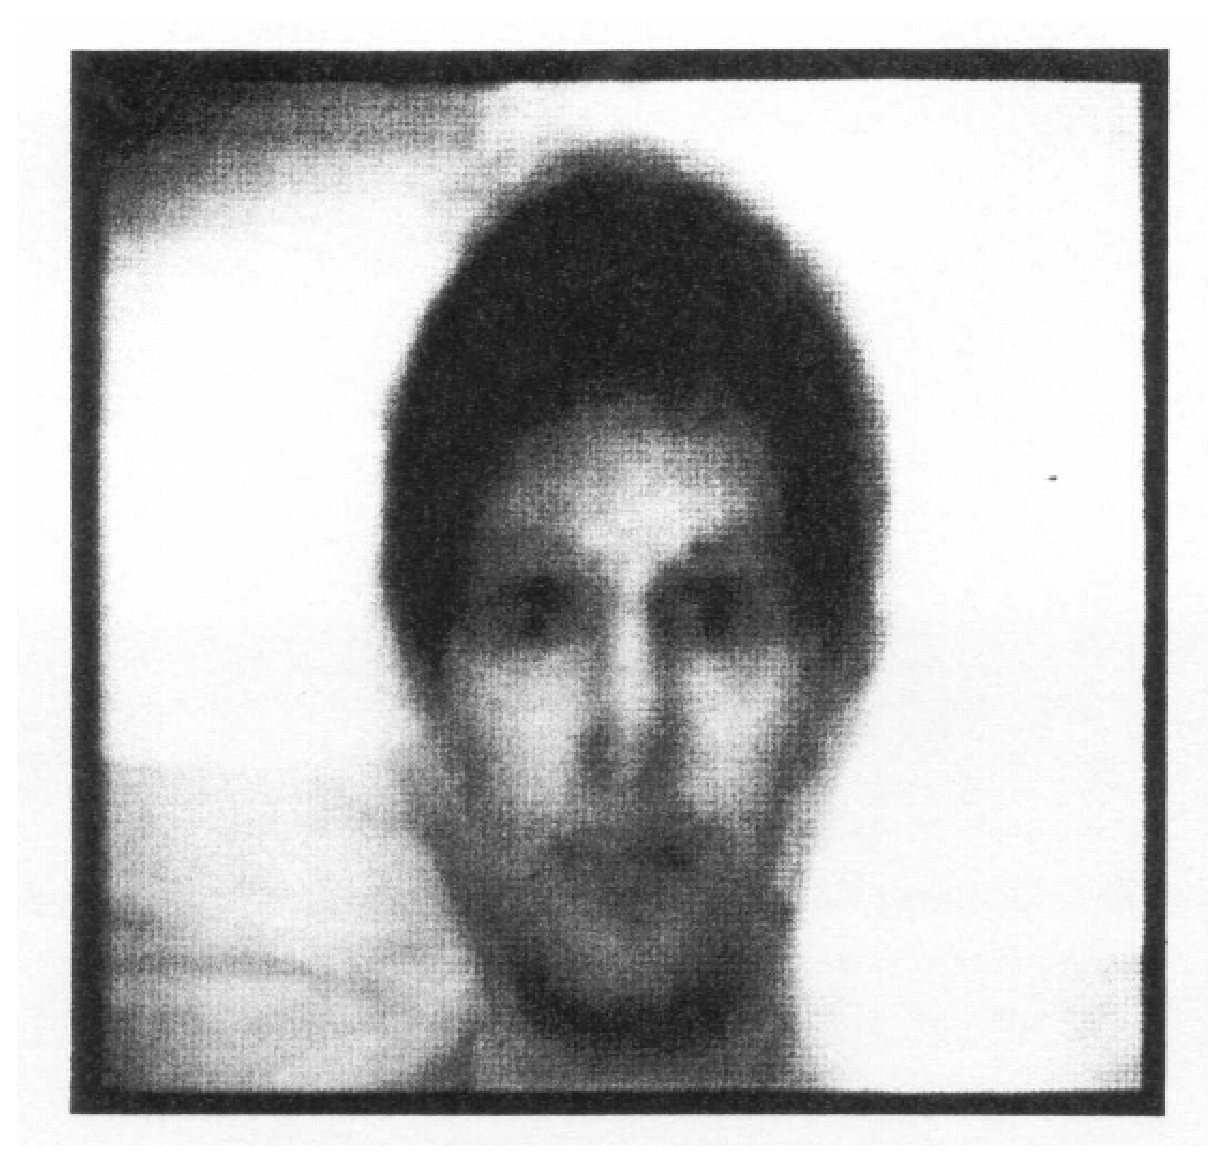
\includegraphics[angle=0,width=0.8\textwidth]{figures/averageFace.eps}
\caption{平均脸}
\end{figure}

\subsubsection{三级标题}
\subsubsection{三级标题}

\newpage
\section{第三章}

\newpage
\section{第四章}

\newpage
\section{结论}

\newpage
\section{结束语}



\end{document}